%!TEX root = ../report.tex

\chapter{Experimental Setup}

Having applied the theoretical knowledge derived in Section 3 to the ROPOD case
study in Section 4 we have begun to narrow down the options for spatio-temporal
world modeling in this particular case. However, a theoretical comparison will
only suffice for so long. Given the focus ROPOD places on real world
environments it is critical that some operational tests be preformed before
method selection. Not only will these experiments serve as a guide for ROPOD,
but they will also act as a template for the comparison of future
spatio-temporal world modeling techniques.


\section{ Environmental Representation}

Given the complexity and size of the target environment, as seen in Figure
TODO, it is necessary to pair down features of the building
until only the core components remain. The three dynamic environmental
components being target are doors, elevators, and carts that are often strewn
about the hallways and surrounding rooms. Therefore, a model environments have
been designed for simulations to be run on that each contain one of these three key
components. The model environments that have been designed take heavy
influence from the actual environment but some notable changes have been made.
The models have a decreased area and a slightly more simplistic design to
allow for faster model training and path planning. Additionally, extraneous
rooms and hallways have been removed. A comparison between the actual hospital
and the designed model can be seen below.\\TODO add pictures from simulated rooms

\begin{figure}[!htb]
  \centering
  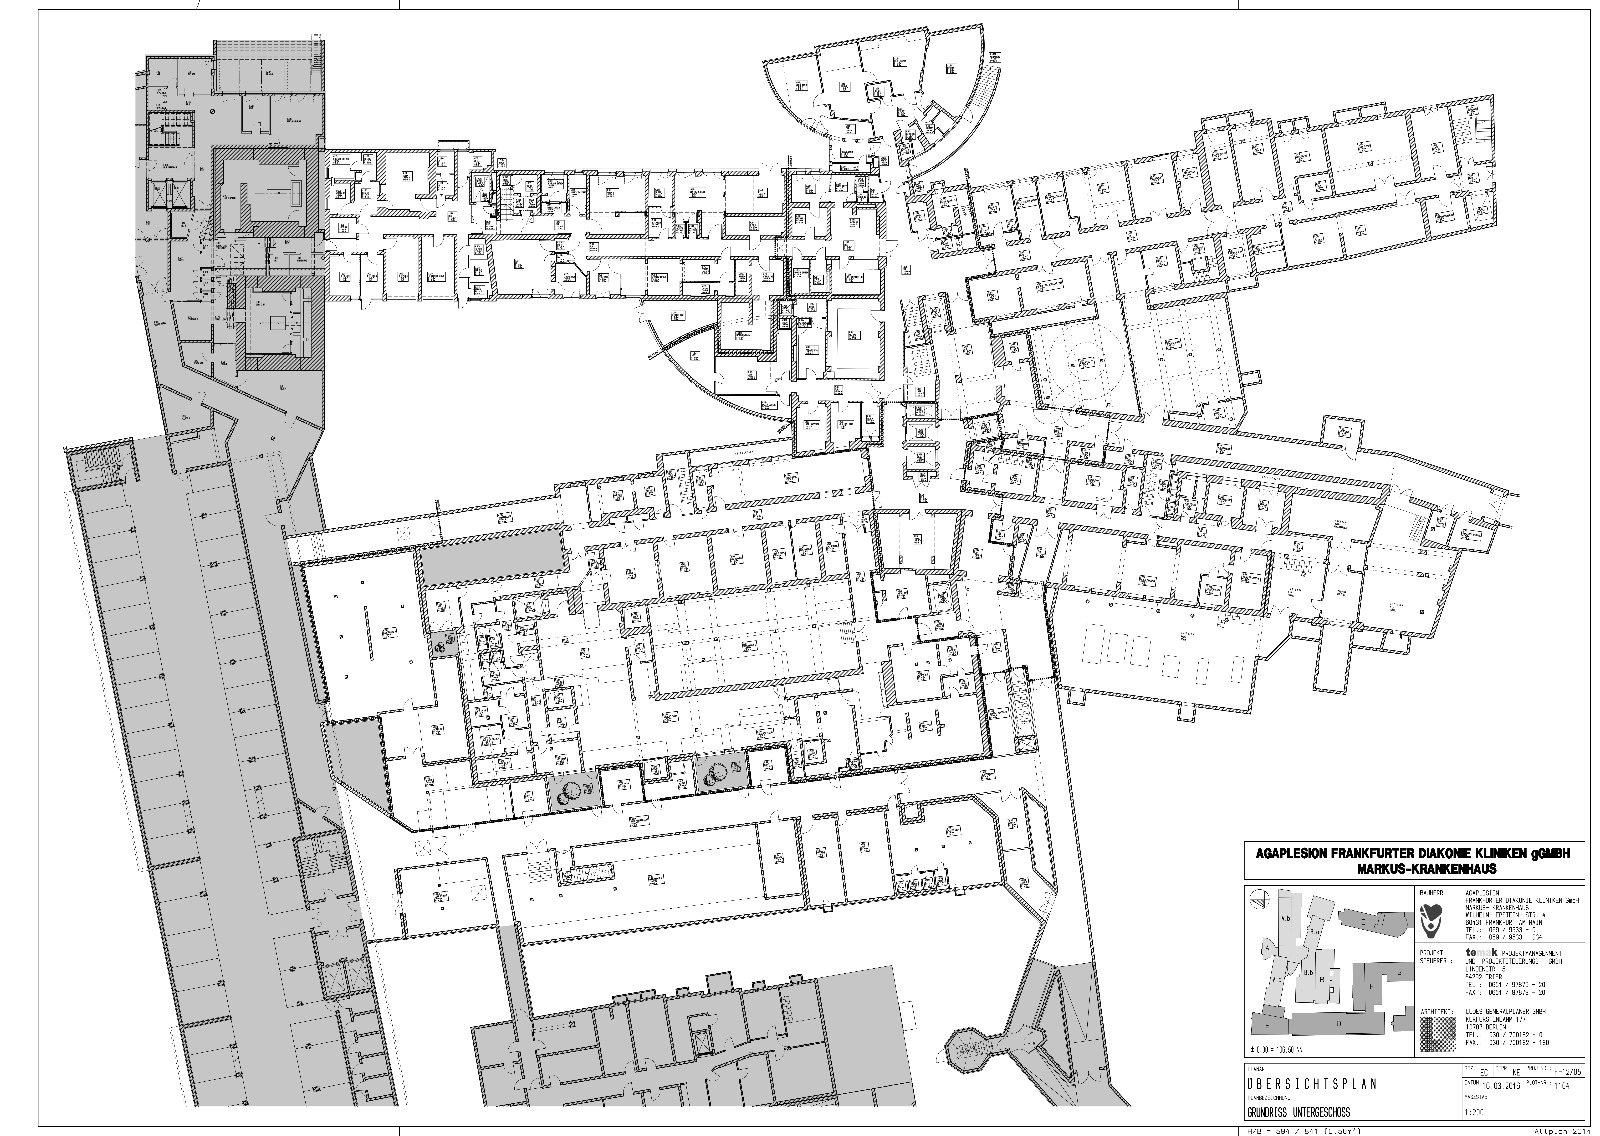
\includegraphics[width=\linewidth]{images/agaplesion_uebersichtsplan.png}
  \caption{One floor of the hospitals layout.}
  \label{figure:hospital_overview}
\end{figure}

\section{ Common Assumptions }
In order to insure only the desired component is being tested at any given
time a set of assumptions are made.

\begin{itemize}

  \item All robot components are working correctly (no internal faults)

  \item Other than the object under test (e.g. doors), all other objects in the
        environment are static

  \item All information other than the objects under test are perfectly known

  \item Observations made/provided by the training data are assumed to be ground-truth

\end{itemize}


\section{ Commonalities in Approach }
Although different components will be under test, each experiment will be run
in a similar manor.

The experimental setup is as follows:

\begin{itemize}

  \item Training data consisting of observations made every 10 minutes over a simulated month will
        be provided to the models

  \item 3 training sets will be made:
    \begin{itemize}

      \item TODO further discuss generation of datasets

      \item Highly consistent generation

      \item Generation consistent with early periodicity of data obtained

      \item Data with higher chance of abnormalities

    \end{itemize}

  \item Using the same generation procedure, a set of three new months will be
        generated

  \item 4 times will be randomly selected each day of the month using a
        uniform distribution for which the models must generate maps

  \item An optimal path using the ground truth will be generated for each of
        these time slots using the selected models

  \item Additionally, maps will be generated using the ground truth, best
        case, and worst case, assumptions

  \item All of these paths will then be compared using the criteria described
        below.

  \item TODO what about a test with sparseness of data

  \item All experiments will be done on the same hardware
    \begin{itemize}
      \item Desktop PC
      \item i7-2600k 3.4GHz
      \item 8GB DDR3
      \item Ubuntu 14.04 Trusty Tahr
    \end{itemize}

\end{itemize}


\section{ Comparison Criteria }
In order to evaluate the intricacies of the selected models a wide variety of
data points have been selected for comparison. A focus has been placed on collecting
data relevant to scale-ability of the modeling technique given the eventual scope of the ROPOD project.

\begin{itemize}

  \item Accuracy to Ground Truth

  \item Accuracy to Historical Recreations

  \item Planning Run-time

  \item Planning Memory Consumption

  \item Size of Generated Model

\end{itemize}


\section{ Doored Areas}

\subsection{ Experimental Motivation }

As is the case in many places of employment many areas of a building may not
be accessible to the public, and by extension the robots, outside of work
hours.  This could come in the form of a given hallway between two areas being
locked after 17:00 as the day works go home. In another case, it could be as
simple as someone preferring to having a door shut to a hallway during a loud
or chaotic time of the day. \\

Regardless of the reason, it is certain that the states of doors are often
both dynamic and periodic. In the ideal case, a robot, much like humans,
would learn when certain doors are closed and be able to plan accordingly.
Making an accurate prediction can save time, but making an inaccurate
predication can also be costly. An in accurate prediction would force a robot
to not only backtrack, but also recalculate that path required to get to a
target. Additionally, it may not be possible to make deliveries at all times.
In the worse case, a robot may even manage to get itself locked in an
environment unable to return back to it's base and eventually run out of power
requiring human intervention. For these reasons and many more, the door
experiment is an excellent example of the benefits of spatio-temporal world
modeling. \\

\subsection{ Experimental Details }

In order to minimize the complexity of the experiment while also maximizing
the value of resulting data the simulation involves only a hallway and three
distinct doors.  Behind each door is a room where a package must be
delivered.  Each model will be directly, or indirectly be tasked with
predicting the state of these door. Door A will represent a door that would be
open during regular work hours, that is to say 9:00-17:00 Monday through
Friday. Door B simulates something close to the inverse of that, a door that
only experiences fluctuations during the workday.  That is to say, from
9:00-17:00 the door is not predictable, i.e. is a random state. Outside of
work hours Monday through Friday, the door is always open. Door C will
simulate a sudden and long term change in the environment. This could be
construction or someone going on an extended vacation. The door will always be
open the first three weeks and then will be closed for the remainder of the
experiment. Figure 5.1 displays the starting and goal points of for desired
paths.


\begin{figure}[!htb]
  \centering
  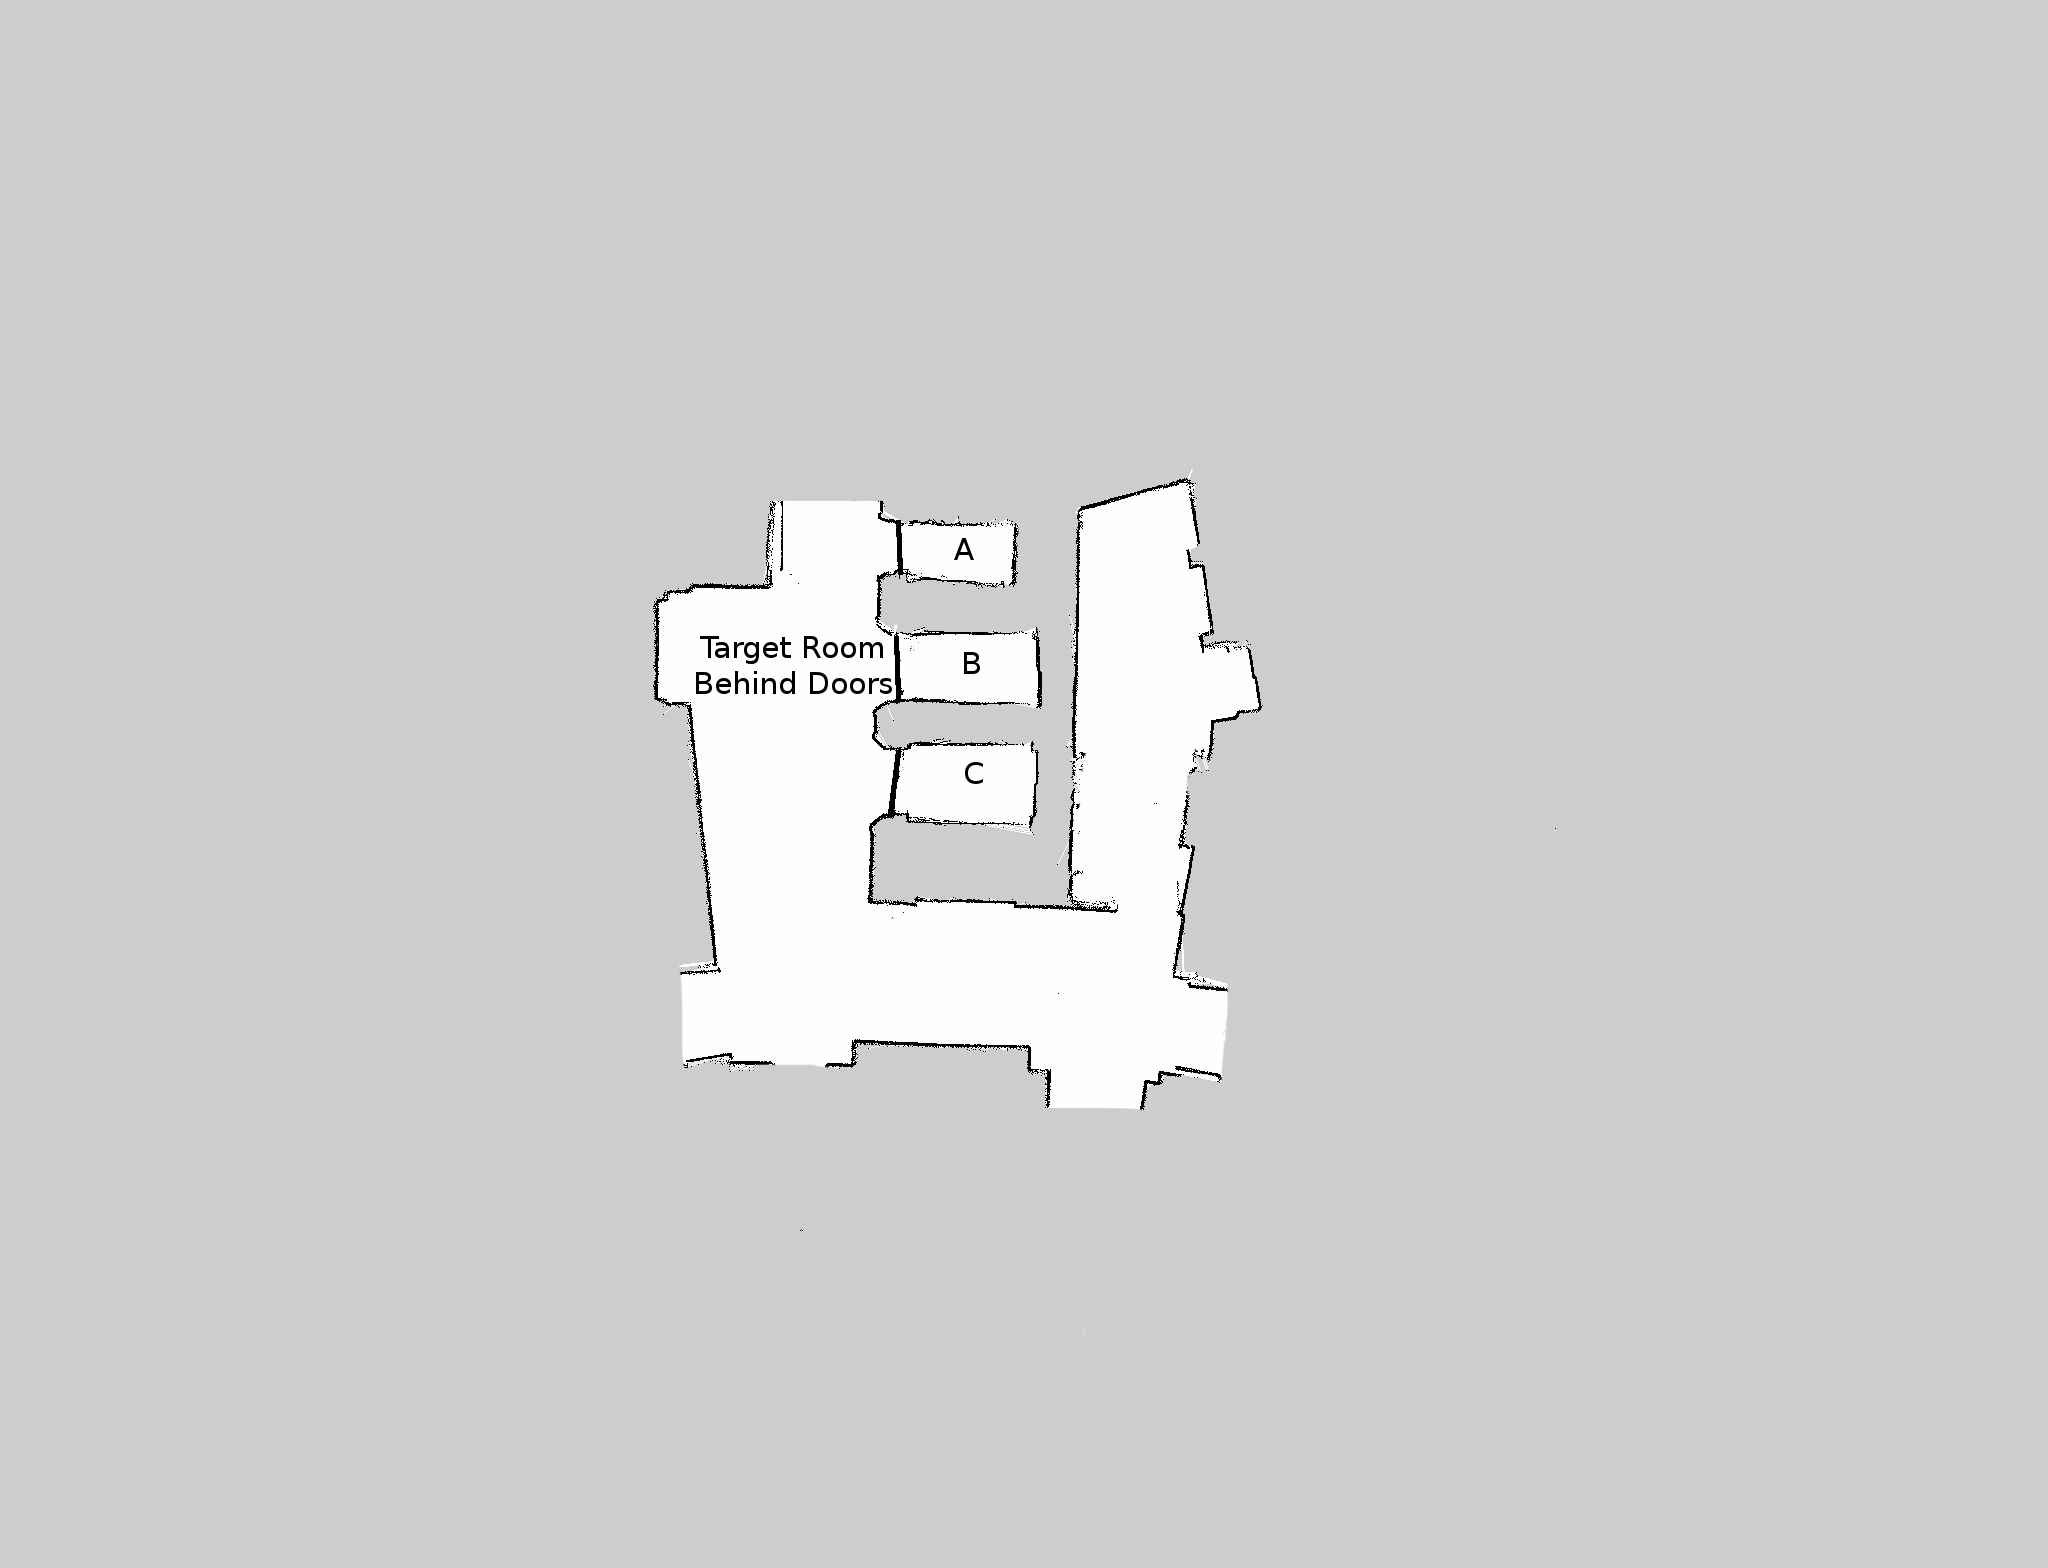
\includegraphics[width=\linewidth]{images/ward_24_door.png}
  \caption{Multiple rooms behind doors in ward 24. }
  \label{figure:ward_24_door}
\end{figure}

TODO should I include something like this here or elsewhere?
A simple 50\% confidence value will be used. That is to say, if a model
predicts that the door will be 50\% or more likely to be open will result in
the robot attempting to deliver the package.  It is clear that this 50\%
cutoff does not take into account the penalties of making a wrong prediction,
but this experiment was designed to investigate the accuracy of the
prediction. How the information of the prediction is handled afterwards is
undoubtedly valuable, but is outside the scope of this current research. \\


\section{ Congested Hallways }

\subsection{ Experimental Motivation }

Hallways, although often seen as an area of high foot traffic, can often serve
a different purpose. When a hallway does not see a lot of foot traffic,
especially from the public, it is common for it to become an area of temporary
storage.  Through use it is common for these storage areas to begin to become
cluttered. This can be seen as a temporary obstacle, but this is also
sometimes periodic behavior. The main goal of this  experiment is to see how
well each of the models deal with objects as they are placed in the hallways.
It does a good job of testing both periodic behavior, as well as temporary
trends in the data.

Figure 5.2 shows the basement of the hospital. This area is used as storage
most often and carts or other objects can build up in the surrounding rooms and
often overflow into the hallways as well. Although it is uncommon, occasionally
it is possible for sections of the hallway to become impassible for a robot.
These areas, although still passible for humans, are not large enough for a
robot carrying equipment to pass safely through.


\subsection{ Experimental Details }

The simulation begins with the robot having already exited the main elevator.
At this point, the models are queried for maps that will be used for planning.
In order to best display and compare the features of the modeling techniques
it is assumed that the hallway on the left, the shorter of the two paths, will
become blocked with a certain frequency. In addition, both hallways may have
objects that will not be easy to traverse, and thus slow the robot down. Much
like the previous experiment, a cell of an occupancy grid, or edge of a graph
with lower than than 50\% chance of being passible will be considered
impassible and thus a different path must be taken.

TODO discussion about occupancy grids vs graphs?



\begin{figure}[!htb]
  \centering
  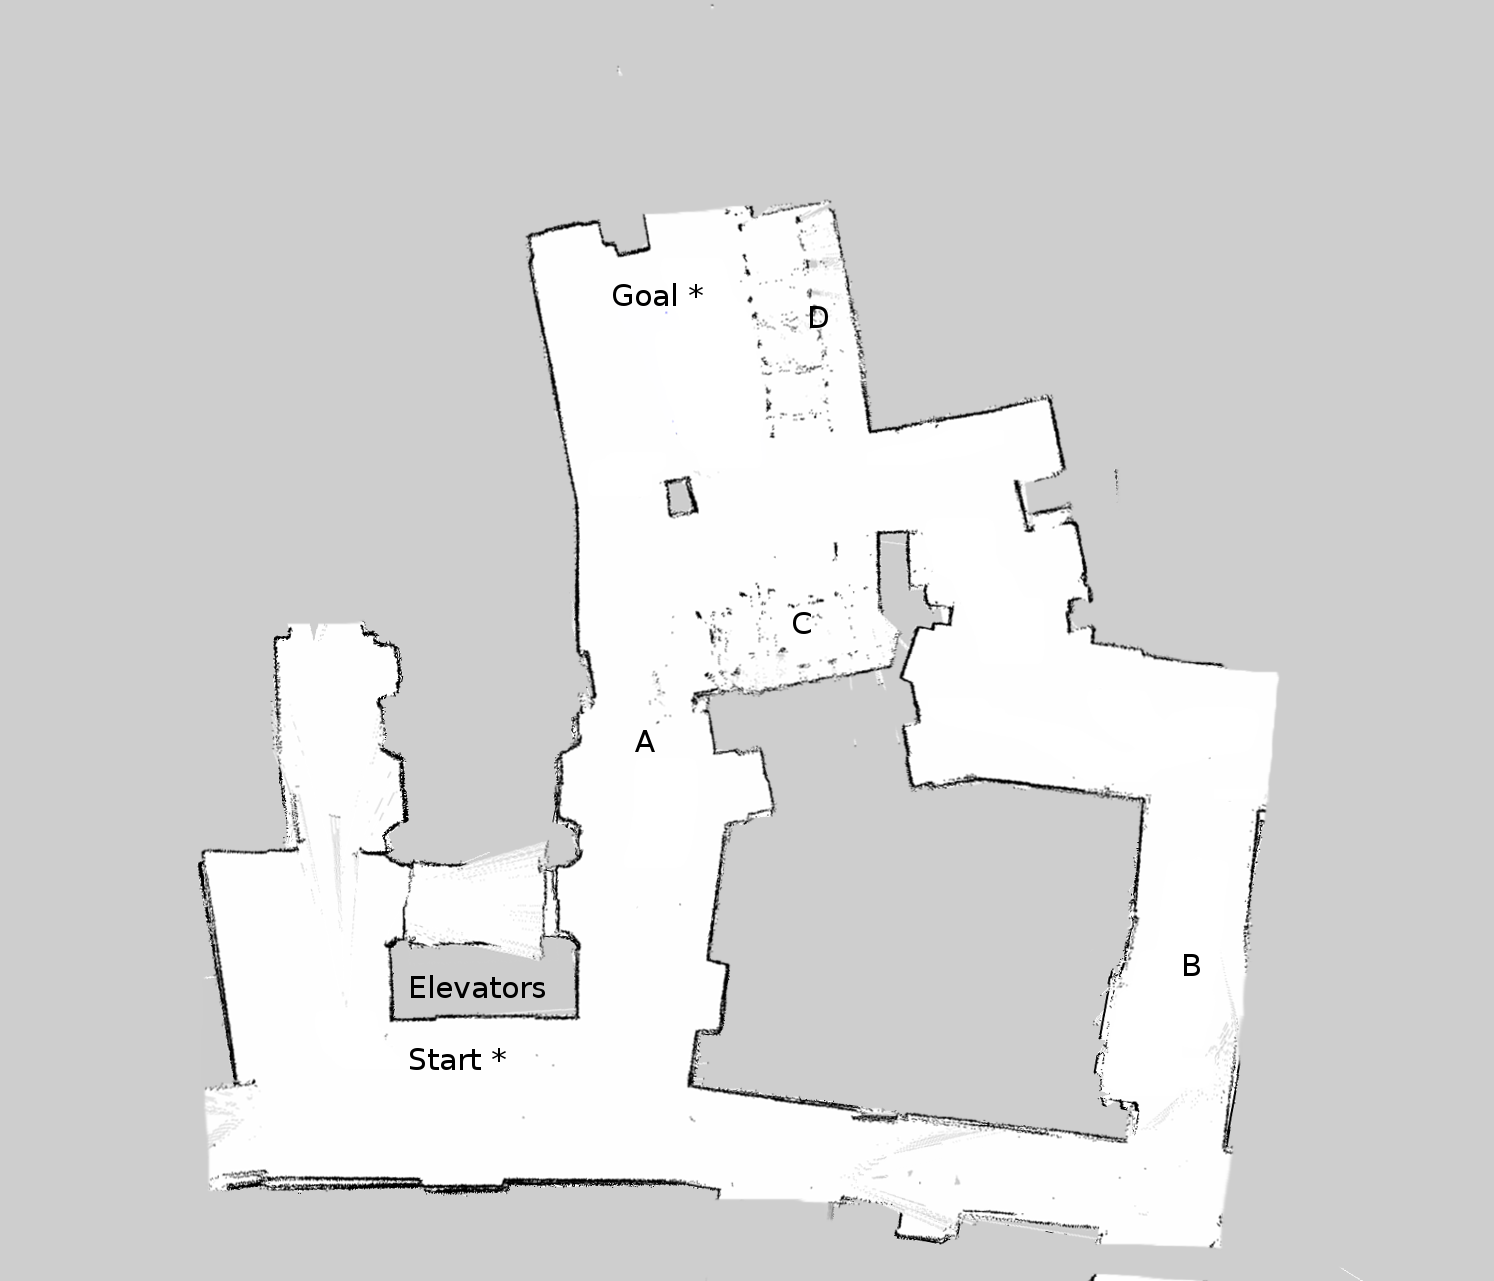
\includegraphics[width=\linewidth]{images/basement_congestion.png}
  \caption{The path from the elevator to the storage area is often congested. }
  \label{figure:basement_congestion}
\end{figure}

The four main areas of notable congestion can be seen in figure 5.3. Area A
can be seen almost of an extension of area C. As C grows larger, objects will
often begin to overflow into the hallway restricting the otherwise shortest
path to the storage area. Furthermore, At times, A can become completely cutoff.
Area B is never seen to be completed congested, and thus is always a safe option,
but there is intermittent and unpredictable foot traffic that may cause disruptions.
C and D are the main areas for storage. C may act as an indicator for A, and
D may occasionally grow large enough to prevent a path to the goal forcing the
robot to go around the pillar (the darker gray square, TODO label).\\

As alluded to above, the simulated areas will act as follows. C and D will start
small as small piles at the beginning of the month growing linearly as the first
two weeks progress before resting back to a small area. This is to simulate the
objects being moved in to permanent storage. Area A will only be affected towards the
last few days before the objects are moved. Since area B is already part of a
longer path, and the foot traffic is fairly limited, it will be assumed area B
is always free and not affected making it a safe, but inefficient choice.



\section{ Busy Elevators }

\subsection{ Experimental Motivation }

The three dimensional nature of human buildings and restrictions caused by
wheeled robots often require that a robot take an elevator to reach it's
destination. This is an extremely common occurrence for ROPOD because the
base station for the robots are situated in the basement. Additionally, these
elevators are not dedicated to ROPOD and are instead shared with the rest of the hospital.
Thus the time between calling an elevator and it arriving can vary. It would
be desirable for ROPOD to be able to predict both at what times the elevators
are busy, and the approximate time it takes to call the elevator.


TODO how to deal with binary restrictions? Another cutoff? Weighted average using confidence value?
Since some of the methods being tested are only able to represent the environment
in terms of binary predictions a work around must be used.

\subsection{ Experimental Details }

The elevators, as mentioned above, will be the only objects that do not easily
map to a binary representation. The elevators, for this simulation will be treated
as a single unit. A few times during the day have been observed as times of peak
use. During these times the elevator has a much higher probability of taking
longer to arrive, or containing people that may hinder the robots ability to enter
the elevator. Peak times for the simulation include an hour before and after
noon, representing the lunch rush and opening hours around 9:00. At these times
a binomial distribution will be used to generate the increase in weight time as
well as the likelihood an elevator is not useable after being called.\\

TODO should I include more specifics and formulas used for the distributions
and such here? Or in the later sections?



\begin{figure}[!htb]
  \centering
  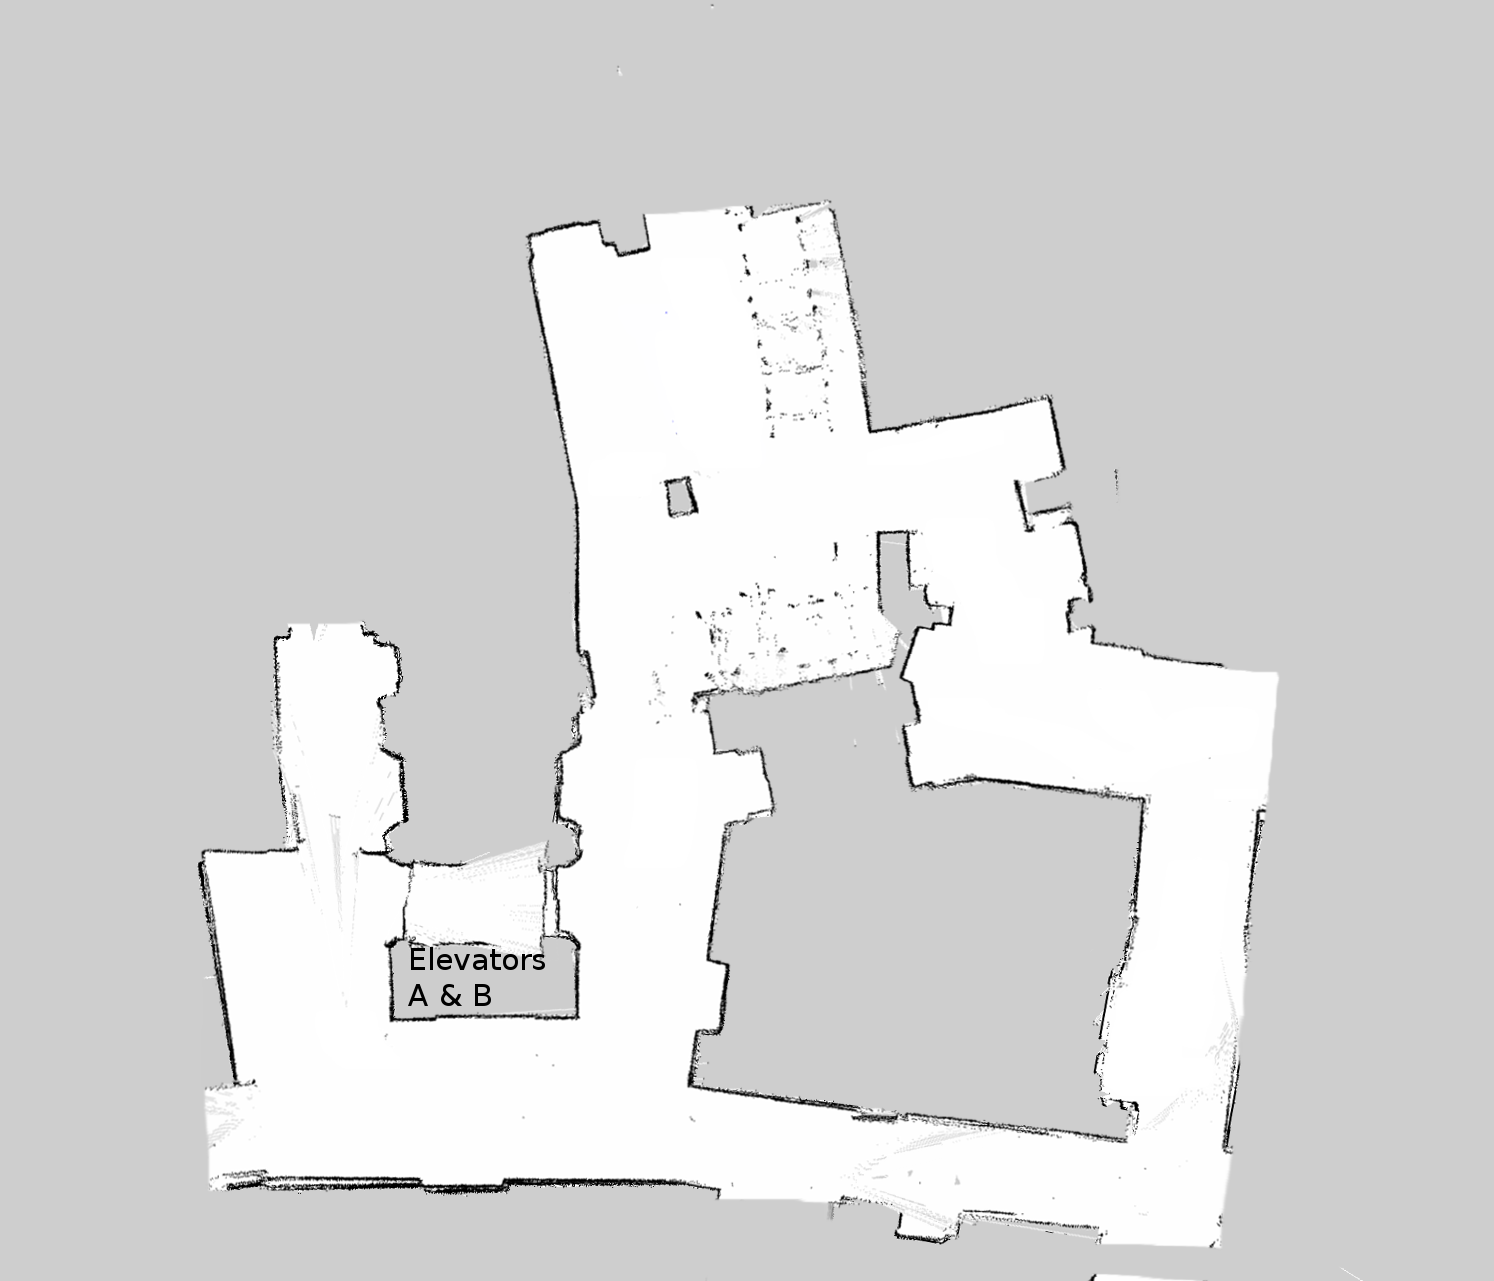
\includegraphics[width=\linewidth]{images/basement_elevator.png}
  \caption{Location of the elevators in the basement. }
  \label{figure:basement_elevator}
\end{figure}
